\section{Алгоритмы и структуры данных}
\subsection{Преобразование цветового пространства (RGB → YCbCr)}

Перед сжатием изображений в формате JPEG зачастую используется преобразование из цветового пространства RGB в YCbCr. 
Это обусловлено как особенностями восприятия цвета человеком, так и требованиями алгоритмов сжатия.


Такое разделение позволяет применить хрома-субдискретизацию — уменьшение разрешения цветовых компонент — без заметного ухудшения качества изображения.
Для RGB с диапазоном значений от 0 до 255, преобразование в YCbCr выполняется по следующим формулам:

$$ Y = 0,299R + 0.587G + 0,114B; $$
$$ Cb = -0,168736R - 0,331264G + 0,5B + 128; $$ 
$$ Cr = 0,5R - 0,418688G - 0,081312B + 128. $$

Здесь значения R, G, B принимаются в диапазоне $[0, 255]$. 
Смещение на 128 единиц в формулах для Cb и Cr необходимо для корректного представления как положительных, так и отрицательных значений в беззнаковом формате (unsigned int).

Поскольку компоненты Cb и Cr менее значимы для восприятия, их можно хранить с пониженным разрешением. 
Наиболее распространённый формат — 4:2:0, при котором на каждые 4 пикселя хранится 4 значения яркости Y и по 1 значению Cb и Cr. 
Это даёт значительное уменьшение объёма данных без существенного ущерба для качества изображения.



\subsection{Преимущества YCbCr}
    \begin{itemize}
        \item Обеспечивает эффективное сжатие без видимых потерь качества;
        \item Разделение яркости и цвета позволяет применять различные методы компрессии к компонентам Y и CbCr;
        \item Поддерживается большинством стандартов обработки изображений и видео.
    \end{itemize}

    Таким образом, преобразование RGB → YCbCr является ключевым шагом в JPEG и других алгоритмах сжатия, 
    позволяющим использовать особенности восприятия цвета человеком для достижения более высокой степени сжатия.




\subsection{Субдискретизация}
На втором этапе сжатия изображения применяется методика, известная как субдискретизация цветности (англ. chroma subsampling). 
Её ключевая идея заключается в сокращении объёма данных, содержащих информацию о цвете, путём уменьшения пространственного разрешения цветовых компонентов. 
Это возможно благодаря физиологической особенности зрительной системы человека: 
она в гораздо большей степени чувствительна к деталям яркости (компонент Y — luminance), чем к изменениям цветовых оттенков (компоненты Cb и Cr — chrominance).

В практической реализации данный метод означает, что цветовая информация (Cr и Cb) кодируется с меньшей точностью по сравнению с яркостной. 
Существует несколько вариантов схем хрома-субдискретизации, которые различаются по степени уменьшения разрешения цветовых компонентов:

4:4:4 — нет сжатия, все компоненты Y, Cb и Cr сохраняют оригинальное разрешение.

4:2:2 — разрешение Cb и Cr уменьшается в два раза по сравнению с Y.

4:2:0 — стандарт для большинства сжатых форматов, где разрешение Cb и Cr уменьшается в два раза как по вертикали, так и по горизонтали.

Схема 4:2:0 является наиболее распространенной для видео и изображений, так как она дает хороший баланс между качеством и сжатием. 
Она предполагает, что на каждые четыре пикселя яркости (расположенных в виде блока 2×2) приходится всего один усреднённый пиксель Cr и один усреднённый пиксель Cb. 
То есть цветовые значения вычисляются как средние значения для группы пикселей, и это значение применяется ко всей группе. 
В результате разрешение цветовых компонентов уменьшается в четыре раза (на 75\%) по сравнению с яркостной компонентой.

Для визуализации можно представить исходное изображение как состоящее из трёх равнозначных слоёв:

Y (яркость),

Cb (синий цветовой компонент),

Cr (красный цветовой компонент).

До субдискретизации каждый из этих компонентов имел одинаковое разрешение и соответственно одинаковый вклад в общий объём данных:

$$
Y + Cb + Cr = 1+1+1=3 \text{ единицы информации}.
$$

После применения схемы 4:2:0, каждая из цветовых компонент уменьшается до $\frac{1}{4}$ исходного размера, а яркостная остаётся без изменений:

$$
Y + \frac{1}{4}Cb + \frac{1}{4}Cr = 1 + 0.25 + 0.25 = 1.5 \text{ единицы информации}.
$$

\begin{figure}[H]
    \centering
    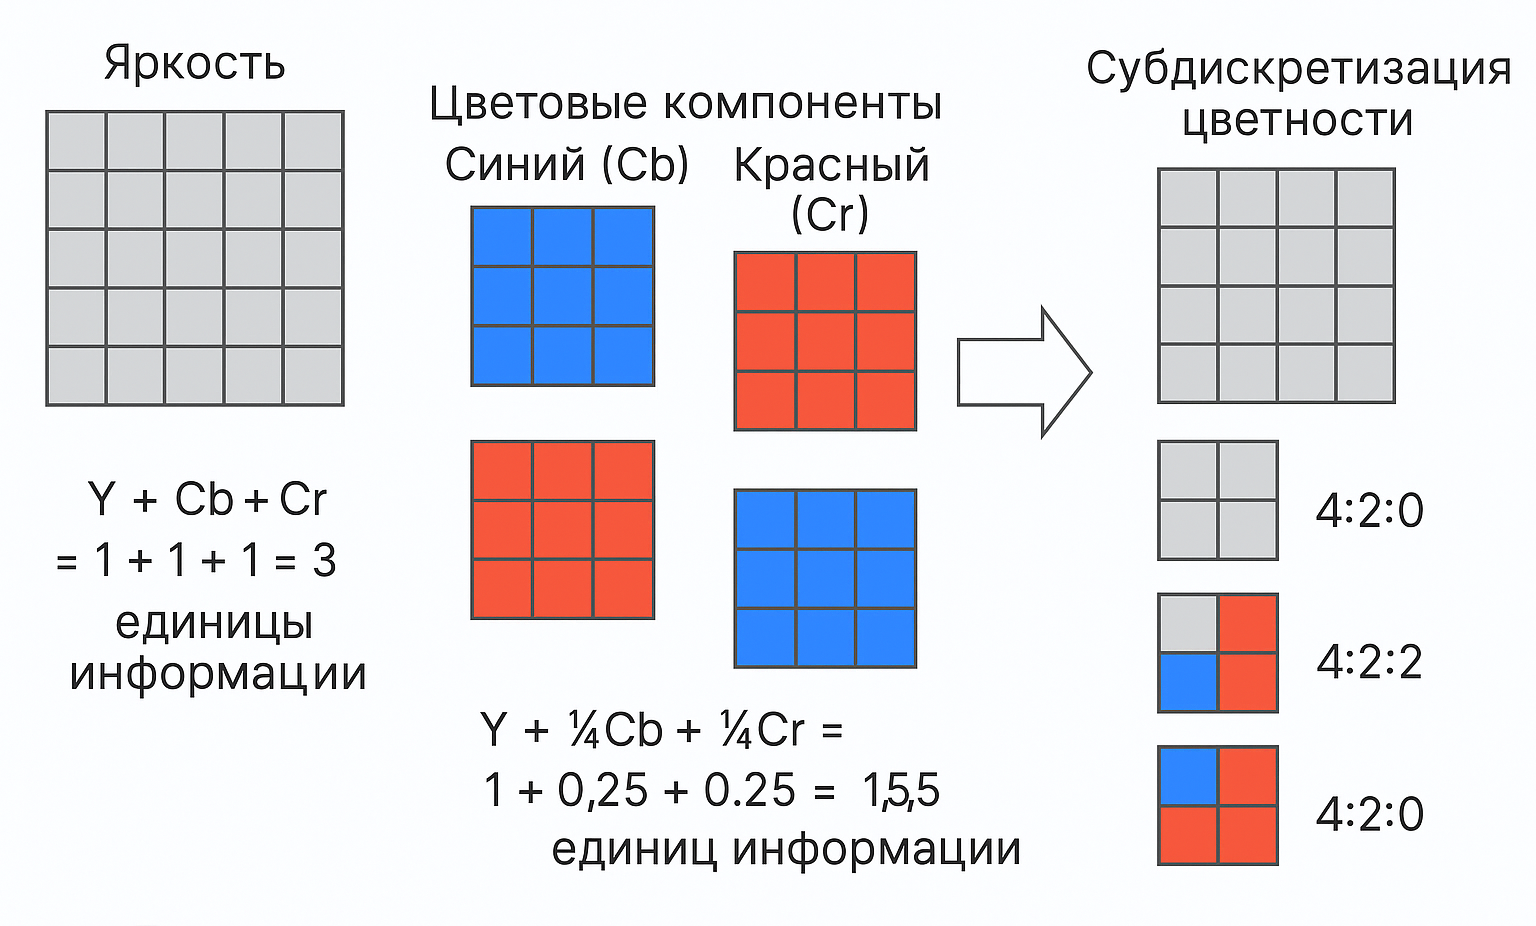
\includegraphics[width=0.7\textwidth]{/home/evgen/Coursework/app/diplom/images/sub_discretization.png}
    \caption{Как происходит преборазование}
    \label{fig:sub_dis}
\end{figure}

Таким образом, достигается двукратное уменьшение общего объёма данных, подлежащих хранению или передаче.

Что важно, такое преобразование происходит практически без визуальных потерь качества. 
Несмотря на то, что цветовые данные редуцируются, человеческий глаз практически не воспринимает различие между оригинальным и сжатым изображением. 
Именно поэтому субдискретизация цветности широко применяется в большинстве алгоритмов сжатия изображений и видео (JPEG, MPEG, H.264),
где критически важно достичь компромисса между качеством и эффективностью хранения данных.


\subsection{Дискретное косинус-преобразование}

После преобразования изображения из цветового пространства RGB в YCbCr и выполнения хрома-субдискретизации (уменьшения разрешения цветовых компонент Cb и Cr), 
выполняется разбиение изображения на блоки фиксированного размера 8×8 пикселей. 
Однако размеры исходного изображения не всегда кратны восьми, что делает невозможным непосредственное и равномерное разбиение без остатка. 
В таких случаях производится предварительная корректировка размеров изображения: вычисляется необходимое количество дополнительных строк и столбцов, 
которые должны быть добавлены к правому и нижнему краю изображения для достижения кратности 8.

Добавление недостающих строк и столбцов осуществляется с помощью повторения граничных значений (пикселей) изображения, 
чтобы минимизировать искажения, возникающие на краях. 

\AddedBlocks

Этот шаг реализуется при помощи библиотеки OpenCV, предоставляющей функцию для симметричного дополнения изображений. 
После этого скорректированное изображение разбивается на непересекающиеся блоки размером 8×8.

\begin{figure}[H]
    \centering
    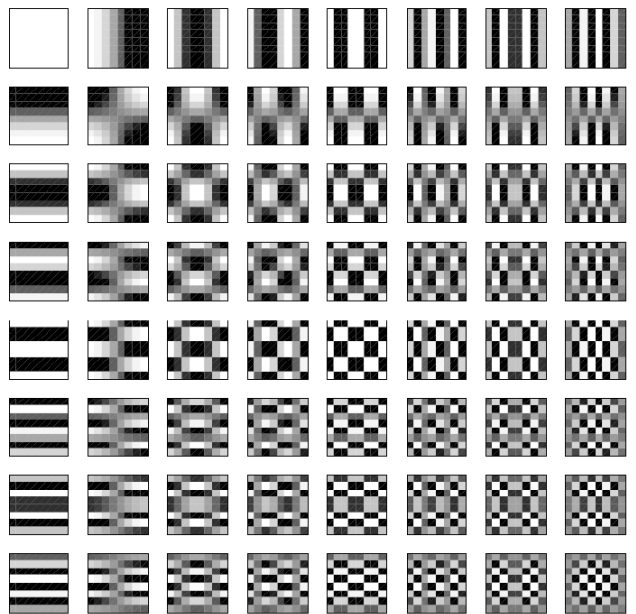
\includegraphics[width=0.7\textwidth]{/home/evgen/Coursework/app/diplom/images/bloks.png}
    \caption{Блоки 8х8}
    \label{fig:blocks}
\end{figure}


Для удобства хранения и последующей обработки эти блоки сохраняются в виде многомерных массивов с использованием библиотеки NumPy. 
Это позволяет эффективно обращаться к отдельным блокам, выполнять над ними математические преобразования и организовать дальнейший процесс.


Это важный шаг, позволяющий значительно повысить эффективность сжатия. 
Разделение на небольшие блоки позволяет применять алгоритмы сжатия локально, что упрощает обработку и улучшает степень компрессии.

Дальнейшая задача заключается в оценке уровня детализации внутри каждого блока. 
Если блок содержит мало визуальных деталей, его можно закодировать с меньшим числом битов, минимизируя потери качества. 
Для анализа степени детализации и выделения значимых компонент используется дискретное косинусное преобразование (ДКП, англ. Discrete Cosine Transform, DCT). 
Преобразование позволяет перейти от пространственного представления блока к частотному, выявляя частотные составляющие, которые имеют наибольшее значение для визуального восприятия.

Для понимания принципов работы ДКП целесообразно сначала рассмотреть его одномерную (векторную) форму, 
поскольку она обладает большей наглядностью и сохраняет все ключевые идеи, лежащие в основе двумерного варианта, применяемого в обработке изображений.
